\chapter{Funzioni ricorsive} \label{ch:capitolo8}
\subsection{Approcci alternativi alla nozione di calcolabilità}
\begin{itemize}
    \item Calcolo equazionale (Gödel,Herbrand,Kleene)
    
    \item lambda-calcolo (Church)
    
    \item funzioni ricorsive parziali (Gödel,Kleene)
    
    \item macchina di Turing
    
    \item sistemi di deduzioni canonici (Post)
    
    \item sistemu di Markov
    
    \item URM (Sheperdson, Sturgis)
\end{itemize}
\textbf{Terorema}\\
Ognuno dei metodi precedenti genera la medesima classe di funzioni
\newpage
\subsection{Funzioni ricorsive di base}
Nel seguito, considereremo esclusivamente funzioni (parziali o totali)
\begin{center}
    $f : N^k \mapsto N$
\end{center}
con $k >= 0$ (l’intero k si dice arietà di f ; nel caso k = 0, f è una costante).\\\\
\textbf{Definizione}\\
Chiameremo funzioni primitive di base le funzioni seguenti.
\begin{enumerate}
    \item La funzione \textbf{successore}
    \begin{center}
        $s$ : $N \mapsto N$ definita da $s(x) = x + 1$
    \end{center}
    \item La funzione \textbf{zero}
    \begin{center}
         $z$ : $N \mapsto N$ definita da $z(x) = 0$
    \end{center}
    \item Le \textbf{proiezioni} 
    \begin{center}
        $P^k_i $ : $N^k \mapsto N $ definita da $P^k_i(x_1,...,x_k) = x_i$ con $1 <= i <= k$
    \end{center}
\end{enumerate}
\subsection{Composizione e recursione}
\textbf{Definizione}\\
Siano $k, n > 0$ con , $h:$ $N^k \mapsto N$ e $g_1,...,g_n:$ $N^k \mapsto N$ funzioni totali.\\
La funzione $f:$ $N^k$ $\mapsto N$ definita da$:$
\begin{center}
    $f(x_1, ... , x_k )= h(g_1(x_1, ... , x_k), ... , g_n(x_1, ... ,x_k))$
\end{center}
si dice la funzione ottenuta per composizione dalle funzioni $h, g_1, ... , g_n$.\\\\
\textbf{Definizione}\\
Sia $k >= 0, h:$ $n^k+2 \mapsto N$ e $g : N^k \mapsto N$ funzioni totali.\\
La funzione $f:N^k+1 \mapsto N$ definita da
\begin{center}
    $f(x_1,..,x_k, 0) = g(x_1,...,x_k)$\\
    $f(x_1,..,x_k, y+1) = h(x_1,...,x_k, y, f(x_1,...,x_k, y)$\\
\end{center}
si dice la funzione ottenuta per \textbf{recursione} dalle funzioni g e h.
\subsection{Funzioni ricorsive primitive}
\textbf{Definizione}\\
Una funzione si dice ricorsiva primitiva se si può ottenere dalle funzioni ricorsive di base con un numero finito di operazioni di composizione e recursione.\\\\
\textbf{Osservazione}\\
Le funzioni ricorsive primitive sono Turing-calcolabili.\\\\
\textbf{Esempi}
\begin{figure}[htp]
    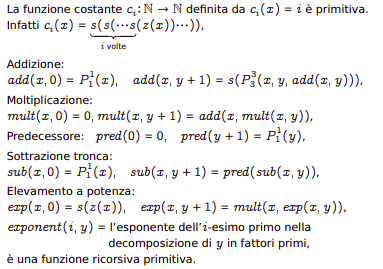
\includegraphics[scale=0.9]{tesi_stile/img/f1cap8.png}
\end{figure}
\newpage
\subsection{La funzione di Ackermann}
\textbf{Problema}\\
La nozione di funzione ricorsiva primitiva coincide con la nozione intuitiva di funzione calcolabile?
\begin{figure}[htp]
    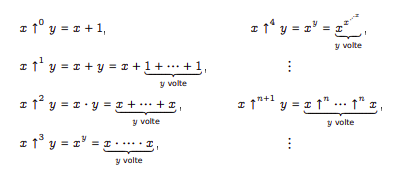
\includegraphics[scale=0.9]{tesi_stile/img/f2cap8.png}
\end{figure}
La funzione $A(n, x) = x \uparrow^n x$ è la funzione di Ackermann.\\
\textbf{Osservazione}\\
\begin{itemize}
    \item La funzione di Ackermann è effettivamente calcolabile
    
    \item cresce molto velocemente
\end{itemize}
\textbf{Teorema}\\
Per ogni funzione ricorsiva primitiva f esiste |$x_0 >= 0$ tale che
\begin{center}
    $f (x) < A(x_1, x_1)$, per ogni $x >= x0$
\end{center}
\textbf{Corollario}\\
La funzione di Ackermann non è ricorsiva primitiva.
\newpage
\subsection{Minimalizzaione}
\textbf{Definizione}\\
Sia $k > 0$ e $g: N^k+1 \mapsto N$ una funzione totale. La funzione parziale $f:N^k \mapsto N$ definita da
\begin{center}
    $f(x_1, ... , x_k ) = min\{y$ | $g(x_1, .. , x_k, y) = 0\}$
\end{center}
si dice ottenuta da g per minimalizzazione.\\\\
\textbf{Osservazione}\\
Se g è calcolabile, allora lo è anche f.\\\\
\textbf{Osservazione}\\
Le nozioni di composizione e recursione si estendono naturalmente alle funzioni parziali.
\subsection{Composizione e recursione}
\textbf{Definizioni}\\
Sia $k > 0$ e $h: N^n \mapsto N$ una funzione ottenuta per composizione dalle funzioni $h_1, g_1,...,g_n$. avrà dominio
\begin{figure}[htp]
    \centering
    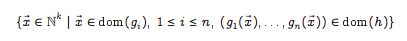
\includegraphics[scale=0.7]{tesi_stile/img/f4cap8.png}
\end{figure}\\
è definito da:
\begin{figure}[htp]
    \centering
    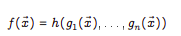
\includegraphics[scale=0.7]{tesi_stile/img/f5cap8.png}
\end{figure}\\
Sia $k >= 0$ , $h: N^{k+2} \mapsto N$ e $g: N^k \mapsto N$  funzioni parziali.\\
La funzione f ottenuta per recursione dalle funzioni g e h avrà dominio definito da
\begin{figure}[htp]
    \centering
    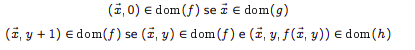
\includegraphics[scale=0.7]{tesi_stile/img/f6cap8.png}
\end{figure}\\
e sarà definito da:
\begin{figure}[htp]
    \centering
    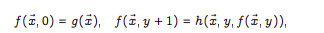
\includegraphics[scale=0.7]{tesi_stile/img/f7cap8.png}
\end{figure}
\newpage
\subsection{Funzioni ricorsive parziali}
\textbf{Definizioni}\\
Una funzione si dice ricorsiva parziale se si può ottenere dalle funzioni
ricorsive di base con un numero finito di operazioni di composizione,
recursione e minimalizzazione.
Si dice funzione ricorsiva una funzione parziale ricorsiva che sia anche
totale.
Infine, un sottoinsieme di N si dice ricorsivo se la sua funzione
caratteristica è ricorsiva.\\\\
\textbf{Proposizione}\\
Le funzioni ricorsive parziali sono calcolabili.
\subsection{Funzioni ricorsive parziali e calcolabilità}
\textbf{Teorema}\\
Una funzione è ricorsiva parziale se e solo se è Turing-calcolabile.\\\\
\textbf{Corollario}\\
Un insieme è ricorsivo se e solo se è decidibile.\\
Diremo che un insieme è ricorsivamente enumerabile se è vuoto o è l’immagine di una funzione ricorsiva.\\\\
\textbf{Corollario}\\
Un insieme è ricorsivamente enumerabile se e solo se è semidecidibile.
\newpage
\subsection{Dimostrazione}
Si è già visto che le funzioni ricorsive parziali sono Turing-calcolabili.
Dobbiamo provare che le funzioni Turing-calcolabili sono ricorsive parziali.
Sia quindi $f$ una funzione Turing-calcolabile e sia $M$ la macchina di Turing che la calcola.
Per ogni descrizione istantanea $C$ di $M$, denoteremo con $gn(C)$ il suo numero di Gödel.\\
Consideriamo le funzioni
\begin{figure}[htp]
    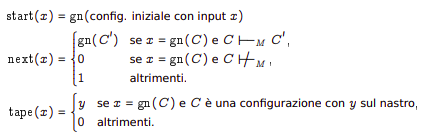
\includegraphics[scale=0.9]{tesi_stile/img/f3cap8.png}
\end{figure}
\newpage
\subsection{Dimostrazione-2}
Le funzioni start, next, tape sono ricorsive primitive. Definiamo $g:N^2 \mapsto N$ con
\begin{center}
    $g(x_1,0) = start(x), g(x ,t+1) = next(g(x_1 ,t)).$
\end{center}
La funzione g calcola il numero di Gödel della configurazione istantanea di M su input x dopo t passi.\\
E' ricorsiva primitiva.\\
La funzione\\
\begin{center}
    $h(x) = min \{t | g(x ,t) = 0\}$
\end{center}
calcola il numero di passi in cui M si arresta su input x , diminuito di 1; è ricorsiva parziale.\\
La funzione\\
\begin{center}
    $k(x) = tape(pred(h(x)$
\end{center}
calcola l’output di $M$ su input x, cioè $f(x)$; è ricorsiva parziale.
